\documentclass[a4paper,12pt]{scrartcl}
\usepackage{amsmath}
\usepackage{amssymb}
\usepackage[UKenglish]{babel}
\usepackage{siunitx}
\usepackage[style=ieee]{biblatex}
\addbibresource{bibliography.bib}
\usepackage[hidelinks]{hyperref}
\usepackage{graphicx}

\graphicspath{{fig/}}

\title{Pre-Design of the Tiltrotor UAV}

\begin{document}
\maketitle
\tableofcontents

\newpage

\section{Requirements}
\begin{itemize}
	\item The UAV shall be able to take off and land vertically.
	\item The UAV shall be able to transition from the vertical flight to the horizontal flight and vice versa.
	\item The UAV shall fit into the Category C0 (privately built)~\cite{tabelle-lba-drohnenfuehrerschein}:
		\begin{itemize}
			\item The UAV shall have a MTOW of less than \SI{250}{\gram}.
			\item The UAV shall have a maximum speed of less than \SI{19}{\metre\per\second}.
		\end{itemize}
	\item 
\end{itemize}

\subsection{Vertical Flight}
\begin{itemize}
	\item Vertical flight only necessary for take-off and landing
	\item No fast manoeuvres necessary
\end{itemize}


\subsection{Horizontal Flight}
\begin{itemize}
	\item The UAV shall be optimized for efficient flight at slow speed.
	\item The manoeuvrability shall suffice for basic manoeuvres. The ability to perform acrobatics is not necessary.
\end{itemize}

\section{Overall Design}
\begin{itemize}
	\item The basic design is a conventional layout with a high wing with a high aspect ratio and a conventional tailplane.
	\item The motors are situated in front and in the back of the wing.
	\item The motors can be turned to perform the transition between vertical and horizontal flight.
	\item The UAV is controlled using a rudder and an elevator. There are no ailerons.
\end{itemize}

\section{Wing Design}

\begin{itemize}
	\item Wing properties:
		\begin{itemize}
			\item High aspect ratio for good efficiency.
			\item Rectangular planform with tapered tips. Reason:
			\item The main part of the wing has no dihedral. Only the wing tips have a moderate dihedral as needed for stability.
		\end{itemize}
	\item Wing surface:
		\[
			S = b_i \cdot l_r + \frac{b-b_i}{2} \cdot \frac{l_r + l_t}{2}
		\]
		\begin{figure}
			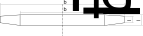
\includegraphics[width = \textwidth]{wing_planform}
			\caption{Wing planform}
			\label{fig:wing-planform}
		\end{figure}
	\item Wing aspect ratio:
		\[
			\Lambda = \frac{b^2}{S}
		\]
	\item Relative mean chord:
		\[
			l_\mu = l_r
		\]
		This is only correct if the wing tips have no sweep.
\end{itemize}

\section{Empennage Design}
\begin{itemize}
	\item The initial sizing of the empennage is done with the formulas given by Raymer~\cite[p. 112]{raymer}.
	\item Both the vertical and horizontal tailplanes have a swept back leading edge and a straight trailing edge.
	\item Length of the mean aerodynamic chord with $\lambda_i = \frac{L_{t,i}}{L_{r,i}}$:
		\[
			L_{\mu, i} = \frac{2}{3} \cdot L_{r,i} \cdot \frac{1 + \lambda_i + \lambda_i^2}{1 + \lambda_i}
		\]
	\item $y$-position of the mean aerodynamic chord:
		\[
			y_{l_{mu},i} = \frac{b_i}{6} \cdot \left( \frac{1+2 \cdot \lambda_i}{1 + \lambda_i}\right)
		\]
\end{itemize}

\subsection{Vertical Tail}
\[
	S_{VT} = \frac{c_{VT} \cdot b \cdot S}{L_{VT}}
\]
\begin{itemize}
	\item The volume coefficient for the vertical tail is chosen as the one of a sailplane ($c_{VT} = 0.02$).
\end{itemize}

\subsection{Horizontal Tail}
\[
	S_{HT} = \frac{c_{HT} \cdot l_\mu \cdot S}{L_{VT}}
\]
\begin{itemize}
	\item The volume coefficient for the horizontal tail is chosen as the one of a sailplane ($c_{VT} = 0.50$).
	\item $L_{VT}$ is the distance of the $\frac{1}{4}$-point of the mean aerodynamic chord of the horizontal tailplane to the centre of gravity.
	\item $l_{mu}$ is the length of the mean aerodynamic chord of the horizontal tailplane.
\end{itemize}

\newpage
\printbibliography


\end{document}
